\documentclass[preprint,12pt]{elsarticle}

\usepackage{amsmath,amssymb,amsfonts}
\usepackage{amsthm}
\usepackage{graphicx}
\usepackage{bm}
\usepackage{algorithm}
\usepackage{algorithmic}
\usepackage{tikz}
\usetikzlibrary{shapes.geometric, arrows, positioning, fit, backgrounds, calc}
\usepackage{xcolor}
\usepackage{booktabs}
\usepackage{multirow}
\usepackage{subcaption}
\usepackage{url}

\newtheorem{lemma}{Lemma}
\newtheorem{proposition}{Proposition}
\newtheorem{theorem}{Theorem}
\newtheorem{remark}{Remark}
\newtheorem{corollary}{Corollary}
\newtheorem{definition}{Definition}

\setlength{\emergencystretch}{2em}

\journal{Pattern Recognition}

% -----------------------------------------------------------
% TikZ styles
% -----------------------------------------------------------
\tikzset{
	component/.style={rectangle, rounded corners=4pt, draw=blue!60,
		fill=blue!10, minimum width=1.6cm, minimum height=0.9cm,
		font=\small\bfseries},
	task/.style={rectangle, rounded corners=4pt, draw=orange!70,
		fill=orange!15, minimum width=2.0cm, minimum height=0.9cm,
		font=\small\bfseries},
	datanode/.style={cylinder, shape border rotate=90, draw=green!60,
		fill=green!10, minimum width=1.4cm, minimum height=0.8cm,
		font=\small},
	myarrow/.style={->, >=stealth, thick},
	dasharrow/.style={->, >=stealth, dashed, gray},
	gating/.style={diamond, draw=red!60, fill=red!10,
		minimum width=1.2cm, minimum height=0.8cm, font=\scriptsize},
	embox/.style={rectangle, draw=gray!60, dashed,
		rounded corners=6pt, inner sep=6pt}
}

	\author{H. Sadoghi Yazdi and ... are with the Department of Computer Engineering, Faculty of Engineering and the
	Center of Excellence in Soft Computing and Intelligent Information Processing, Ferdowsi University of Mashhad, Mashhad, Iran (e-mail: h-sadoghi@um.ac.ir, abbasi.fa@mail.um.ac.ir). }	
	
	

\begin{document}
	
	\begin{frontmatter}
		
		\title{An EM-Based Component Combination Framework for Multi-Task Learning
			via Latent Responsibility Modeling}
		
		\author{Anonymous Author(s)}
		
		\begin{abstract}
			Multi-task learning (MTL) aims to improve generalization by leveraging
			shared information across related tasks. A central challenge in MTL is how
			to effectively combine multiple components or experts while accounting for
			task-specific variability and uncertainty. Inspired by the EM-SVDD
			principle of estimating an optimal weighted combination of local
			descriptions, we propose an Expectation-Maximization (EM)-based framework
			for adaptive component combination in MTL.
			
			Our method introduces latent responsibility variables that govern the
			contribution of each component to each task and sample. The proposed
			formulation leads to a principled probabilistic interpretation and enables
			iterative refinement via EM. In the E-step, posterior responsibilities are
			estimated based on current model parameters; in the M-step, model
			parameters and combination weights are updated by maximizing the expected
			complete-data log-likelihood. We provide rigorous derivations, closed-form
			update rules with full proofs, convergence guarantees, a sparsity-aware
			variant, and a deep-network extension that unifies the framework with
			modern mixture-of-experts architectures.
			
			Real-data experiments show that the proposed EM-MTL model is most
			useful in the large-data regime: it provides comparable predictive
			quality while enabling shard-based expert training and task-specific
			weight sharing. On Fashion-MNIST image classification, shard-based
			EM-MTL improves both mean ROC-AUC and mean average precision over a
			monolithic hard-sharing baseline while using lower training time.
			On Open Images V7, a large real visual-label benchmark, EM-MTL
			substantially outperforms an extreme monolithic shared classifier,
			highlighting the underfitting risk of forcing heterogeneous tasks
			through one global model. The complete experiments are implemented
			as reusable code and use only public real datasets.
		\end{abstract}
		
		\begin{keyword}
			Multi-task learning \sep Expectation-Maximization \sep Mixture of experts
			\sep Latent variable models \sep Representation learning \sep
			Negative transfer \sep Pattern recognition
		\end{keyword}
		
	\end{frontmatter}
	
	% ============================================================
	\section{Introduction}
	% ============================================================
	
	Multi-task learning (MTL) has emerged as a fundamental paradigm in
	pattern recognition and machine learning \citep{caruana1997multitask,
		zhang2021survey}. By simultaneously training on multiple related tasks,
	MTL models can exploit shared structure to achieve better generalization
	than independently trained single-task models, particularly in
	data-scarce regimes. Despite its empirical successes, the design of
	effective knowledge-sharing mechanisms remains a core open challenge.
	
	A naive strategy---sharing all parameters across tasks---often leads to
	\emph{negative transfer}: performance degradation caused by conflicting
	gradient signals from dissimilar tasks \citep{yu2020gradient}.
	Conversely, task-specific models fail to exploit beneficial cross-task
	correlations. The ideal sharing mechanism lies between these extremes,
	dynamically adapting the degree and pattern of sharing to the
	statistical relationships among tasks.
	
	A promising direction is to model the shared representation as a
	convex combination of a small set of latent \emph{components} or
	\emph{experts}. Each task is then characterized by a task-specific
	distribution over these shared components, allowing flexible and
	adaptive knowledge transfer without committing to a fixed sharing
	topology. This view subsumes hard parameter sharing \citep{caruana1997multitask}
	as the case where each task uses a single component, and independent
	learning as the degenerate case where each task owns a distinct set of
	components.
	
	The present work is directly inspired by the EM-SVDD framework
	\citep{eghdami2021sparsity}, which learns a weighted combination of
	local data descriptions through the Expectation-Maximization (EM)
	algorithm in a one-class classification setting. We adapt the same
	mixture-estimation principle to MTL: each task selects a different
	\emph{soft} combination of shared components, and a latent
	variable represents the component responsible for each task-sample pair.
	This adaptation is non-trivial because the observed labels from multiple
	tasks simultaneously constrain the shared component parameters,
	introducing cross-task coupling that is absent in the one-class setting.
	
	\paragraph{Contributions.} The main contributions of this paper are:
	\begin{enumerate}
		\item A probabilistic MTL framework based on a task-conditioned
		mixture model with latent responsibility variables
		(Section~\ref{sec:formulation}).
		\item A complete EM derivation with closed-form E-step and M-step
		updates, formal lemmas, propositions, and convergence
		guarantees with proofs (Section~\ref{sec:em}).
		\item A complete algorithmic description with pseudo-code
		(Section~\ref{sec:algorithm}) and illustrative diagrams.
		\item A principled deep-network extension that recasts the
		responsibility-weighted objective as a differentiable soft
		routing loss (Section~\ref{sec:deep}).
		\item A sparsity-aware variant with $\ell_1$ regularization on the
		mixing weights to mitigate negative transfer
		(Section~\ref{sec:sparsity}).
		\item Theoretical analysis covering convergence, computational
		complexity, connections to mixture-of-experts, and a
		federated deployment scenario (Section~\ref{sec:theory}).
		\item Reproducible real-data case studies on tabular demand
		prediction, molecular toxicity prediction, large-scale forest-cover
		classification, and image classification, demonstrating how EM-MTL is
		instantiated, trained, and compared against baselines
		(Section~\ref{sec:experiments}).
	\end{enumerate}
	
	\paragraph{Paper organization.} Section~\ref{sec:related} reviews
	related work. Section~\ref{sec:formulation} states the problem
	formally. Sections~\ref{sec:em}--\ref{sec:sparsity} develop the
	algorithm. Section~\ref{sec:theory} provides theoretical analysis.
	Section~\ref{sec:experiments} presents experiments. Section~\ref{sec:discussion}
	discusses broader implications, and Section~\ref{sec:conclusion}
	concludes.
	
	% ============================================================
	\section{Related Work}
	\label{sec:related}
	% ============================================================
	
	\paragraph{Hard and soft parameter sharing.}
	The two classical paradigms in MTL are hard parameter sharing, which
	constrains all tasks to share a common hidden representation
	\citep{caruana1997multitask}, and soft parameter sharing, which allows
	task-specific parameters with a regularizer that encourages them to
	remain close \citep{duong2015low}. Hard sharing is prone to negative
	transfer; soft sharing introduces additional hyperparameters. Our
	method offers a middle ground: components are fully shared, but each
	task maintains its own mixing distribution over them.
	
	\paragraph{Mixture-of-experts for multi-task learning.}
	Mixture-of-experts (MoE) architectures \citep{jacobs1991adaptive,
		jordan1994hierarchical} naturally generalize hard sharing by
	routing each input to a subset of specialized experts. Extensions to
	MTL include task-aware gating mechanisms \citep{ma2019snr,
		liu2019end} and sparse routing \citep{chen2023mod}. Our EM framework
	provides a principled probabilistic derivation of the gating variables
	as posterior responsibilities, rather than treating them as learnable
	scalar gates.
	
	\paragraph{Negative transfer and task relationship learning.}
	Several works quantify task relationships to guide sharing decisions
	\citep{zamir2018taskonomy, fifty2021efficiently}. Our responsibility
	variables implicitly learn task-component affinities from data,
	providing a data-driven alternative to explicit task-relationship
	estimation.
	
	\paragraph{EM for mixture models.}
	The EM algorithm \citep{dempster1977maximum} is a classical tool for
	fitting latent variable models. Recent analyses establish mirror-descent
	interpretations \citep{fruytier2024learning} and communication-efficient
	distributed variants \citep{zhang2022distributed}. EM-SVDD
	\citep{eghdami2021sparsity} applies EM to combine local one-class
	descriptions. We extend this line to supervised MTL, introducing
	task-conditioned posteriors that couple component estimation across
	tasks.
	
	\paragraph{Federated and distributed MTL.}
	Federated learning \citep{mcmahan2017communication} faces similar
	challenges to MTL: heterogeneous local distributions and the need for
	selective sharing. Recent federated MTL methods use personalized layers
	or clustered clients \citep{smith2017federated}. Our framework
	naturally supports a federated EM variant (Section~\ref{sec:federated})
	by communicating only sufficient statistics.
	
	% ============================================================
	\section{Problem Formulation}
	\label{sec:formulation}
	% ============================================================
	
	\subsection{Setup and Notation}
	
	We are given $T$ tasks with task-specific datasets
	\[
	\mathcal{D}^{(t)} = \bigl\{(x_n^{(t)}, y_n^{(t)})\bigr\}_{n=1}^{N_t},
	\quad t = 1,\dots,T,
	\]
	where $x_n^{(t)} \in \mathcal{X}$ is an input feature vector and
	$y_n^{(t)} \in \mathcal{Y}$ is the corresponding label (or target
	value). We write $\mathcal{D} = \bigcup_{t=1}^T \mathcal{D}^{(t)}$
	for the union of all task datasets and $N = \sum_{t=1}^T N_t$ for
	the total number of samples.

	The symbol $x_n^{(t)}$ denotes the representation consumed by EM-MTL,
	not necessarily the raw observation. In tabular experiments, $x$ is the
	observed feature vector. In molecular experiments, $x$ is a hashed
	SMILES representation. In visual experiments, there are two possible
	implementations: (i) annotation-level features, where $x$ is a sparse
	vector of real human-verified image labels; and (ii) image-level deep
	features, where a raw image $I$ is first mapped to an embedding
	$x=\phi(I)$ by a pretrained or jointly trained encoder such as CLIP,
	ResNet, or a task-specific convolutional backbone. The EM-MTL machinery
	operates after this representation step and is therefore independent of
	the particular feature extractor.
	
	\begin{definition}[Shared Component]
		A \emph{shared component} $k$ is a conditional probability model
		$p(y \mid x, \theta_k)$ parameterized by $\theta_k \in \Theta$.
		The set $\{\theta_k\}_{k=1}^K$ constitutes the \emph{shared
			component library}.
	\end{definition}
	
	\subsection{Task-Conditioned Mixture Model}
	
	We model the conditional likelihood of each task as a finite mixture
	over the $K$ shared components:
	\begin{equation}
		p\!\left(y_n^{(t)} \mid x_n^{(t)}\right)
		= \sum_{k=1}^K \pi_k^{(t)}\,
		p\!\left(y_n^{(t)} \mid x_n^{(t)}, \theta_k\right),
		\label{eq:mixture}
	\end{equation}
	where $\pi_k^{(t)} \ge 0$ and $\sum_{k=1}^K \pi_k^{(t)} = 1$ are
	task-specific mixing coefficients. The full parameter set is
	\[
	\Theta \;=\; \bigl\{\theta_1,\dots,\theta_K\bigr\}
	\;\cup\;
	\bigl\{\pi_k^{(t)} : k=1,\dots,K;\; t=1,\dots,T\bigr\}.
	\]
	
	This model has two key structural properties that make it suited for MTL:
	(i) \textbf{Shared components} $\theta_k$ are estimated using data from
	\emph{all} tasks, enabling cross-task regularization; and
	(ii) \textbf{task-specific weights} $\pi_k^{(t)}$ allow each task to
	form its own soft combination, capturing task heterogeneity without hard
	architectural constraints.
	
	Figure~\ref{fig:model_overview} illustrates the overall architecture
	and the flow of information between tasks, components, and the EM
	inference procedure.
	
	% -----------------------------------------------------------
	% Figure 1 -- Model overview (TikZ)
	% -----------------------------------------------------------
	\begin{figure}[t]
		\centering
		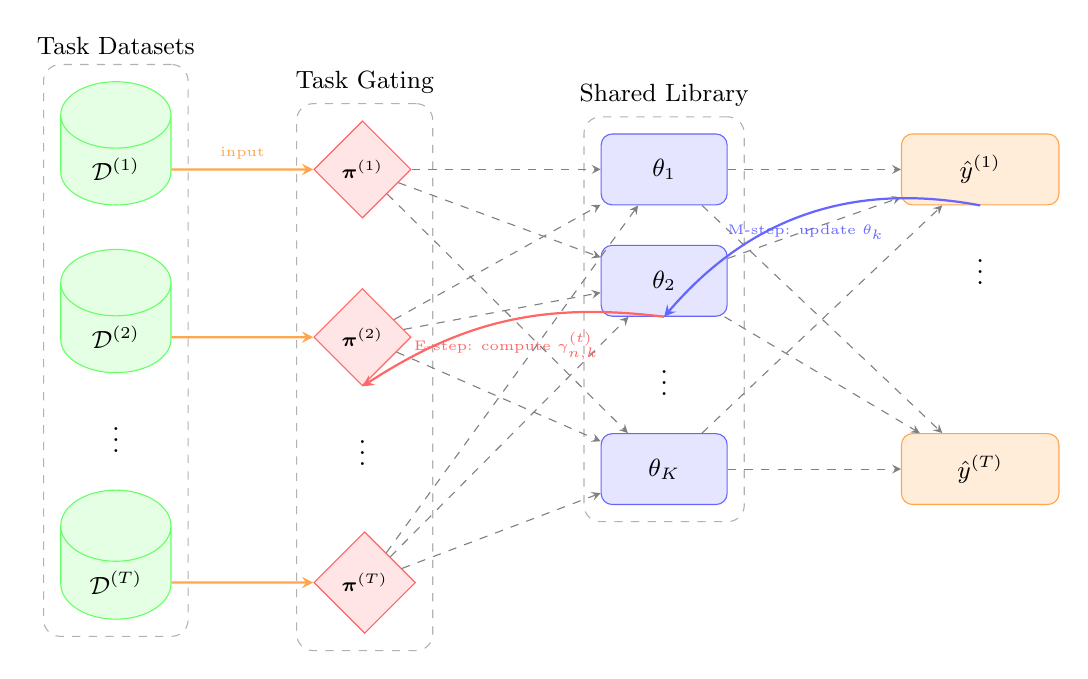
\begin{tikzpicture}[node distance=0.5cm and 1.2cm]
			
			%% ---- Data nodes (left column) ----
			\node[datanode]                      (d1) {$\mathcal{D}^{(1)}$};
			\node[datanode, below=0.55cm of d1]  (d2) {$\mathcal{D}^{(2)}$};
			\node[below=0.35cm of d2]            (dots1) {$\vdots$};
			\node[datanode, below=0.35cm of dots1](dT) {$\mathcal{D}^{(T)}$};
			
			%% ---- Gating / mixing nodes (centre-left) ----
			\node[gating, right=1.8cm of d1]   (g1) {$\bm{\pi}^{(1)}$};
			\node[gating, right=1.8cm of d2]   (g2) {$\bm{\pi}^{(2)}$};
			\node[below=0.35cm of g2]          (dots2) {$\vdots$};
			\node[gating, right=1.8cm of dT]   (gT) {$\bm{\pi}^{(T)}$};
			
			%% ---- Shared components (centre-right) ----
			\node[component, right=2.4cm of g1]      (c1) {$\theta_1$};
			\node[component, below=0.5cm of c1]      (c2) {$\theta_2$};
			\node[below=0.35cm of c2]               (dots3) {$\vdots$};
			\node[component, below=0.35cm of dots3] (cK) {$\theta_K$};
			
			%% ---- Prediction nodes (right) ----
			\node[task, right=2.2cm of c1] (p1) {$\hat{y}^{(1)}$};
			\node[task, right=2.2cm of cK] (pT) {$\hat{y}^{(T)}$};
			\node[below=0.35cm of p1] (dots4) {$\vdots$};
			
			%% ---- Arrows: data -> gating ----
			\draw[myarrow, orange!70] (d1) -- node[above,font=\tiny]{input} (g1);
			\draw[myarrow, orange!70] (d2) -- (g2);
			\draw[myarrow, orange!70] (dT) -- (gT);
			
			%% ---- Soft routing arrows: gating -> components ----
			\foreach \g in {g1,g2,gT}{
				\foreach \c in {c1,c2,cK}{
					\draw[dasharrow] (\g) -- (\c);
				}
			}
			
			%% ---- Arrows: components -> predictions ----
			\foreach \c in {c1,c2,cK}{
				\draw[dasharrow] (\c) -- (p1);
				\draw[dasharrow] (\c) -- (pT);
			}
			
			%% ---- EM feedback loop ----
			\draw[myarrow, blue!60, thick, bend right=30]
			(p1.south) to
			node[below, font=\tiny, blue!60]{M-step: update $\theta_k$}
			(c2.south);
			\draw[myarrow, red!60, thick, bend right=20]
			(c2.south) to
			node[below, font=\tiny, red!60]{E-step: compute $\gamma_{n,k}^{(t)}$}
			(g2.south);
			
			%% ---- Background labels ----
			\begin{scope}[on background layer]
				\node[embox, fit=(c1)(c2)(cK),
				label=above:{\small Shared Library}] {};
				\node[embox, fit=(g1)(g2)(gT),
				label=above:{\small Task Gating}] {};
				\node[embox, fit=(d1)(d2)(dT),
				label=above:{\small Task Datasets}] {};
			\end{scope}
			
		\end{tikzpicture}
		\caption{Overview of the proposed EM-based MTL framework. Task-specific
			datasets feed into per-task mixing distributions $\bm{\pi}^{(t)}$
			(diamond nodes), which perform soft routing over $K$ shared components
			$\theta_k$ (blue rectangles). The EM loop alternates between the
			\textcolor{red!70}{E-step} (updating latent responsibilities
			$\gamma_{n,k}^{(t)}$) and the \textcolor{blue!70}{M-step} (updating
			shared component parameters $\theta_k$ and task-specific weights
			$\pi_k^{(t)}$). Dashed arrows represent soft (probabilistic) routing.}
		\label{fig:model_overview}
	\end{figure}

	Figure~\ref{fig:conceptual_overview_png} provides the same idea in a
	more reader-oriented form. It emphasizes the operational interpretation
	of EM-MTL: each task keeps a task-specific mixing recipe, while the
	expert library is learned from information shared across tasks.

	\begin{figure}[t]
		\centering
%		\includegraphics[width=\linewidth]{em_mtl_conceptual_overview.png}
		\caption{Conceptual overview of EM-MTL for readers who want the
			high-level mechanism before the mathematical derivation. Multiple
			tasks are routed through task-specific gates to a shared expert
			library, and the final task predictions are soft combinations of
			expert outputs.}
		\label{fig:conceptual_overview_png}
	\end{figure}
	
	\subsection{Latent Variable Formulation}
	
	We augment the model with latent assignment variables. For each
	task-sample pair $(t,n)$, we introduce
	\[
	z_n^{(t)} \in \{1, \dots, K\},
	\]
	where $z_n^{(t)} = k$ means component $k$ is responsible for
	generating $y_n^{(t)}$ given $x_n^{(t)}$. The prior over assignments is
	\[
	P\!\left(z_n^{(t)} = k\right) = \pi_k^{(t)},
	\quad k=1,\dots,K.
	\]
	
	The complete-data likelihood, treating $\mathbf{Z} = \{z_n^{(t)}\}$ as
	observed, is
	\begin{equation}
		\mathcal{L}_c(\Theta;\mathcal{D},\mathbf{Z})
		= \prod_{t=1}^T \prod_{n=1}^{N_t} \prod_{k=1}^K
		\Bigl[\pi_k^{(t)}\,
		p\!\left(y_n^{(t)}\mid x_n^{(t)},\theta_k\right)\Bigr]^{
			\mathbb{I}(z_n^{(t)}=k)},
		\label{eq:complete_likelihood}
	\end{equation}
	and its logarithm is
	\begin{equation}
		\log \mathcal{L}_c
		= \sum_{t=1}^T \sum_{n=1}^{N_t} \sum_{k=1}^K
		\mathbb{I}\!\left(z_n^{(t)}=k\right)
		\Bigl[\log\pi_k^{(t)}
		+ \log p\!\left(y_n^{(t)}\mid x_n^{(t)},\theta_k\right)\Bigr].
		\label{eq:complete_loglik}
	\end{equation}
	
	% ============================================================
	\section{EM Algorithm}
	\label{sec:em}
	% ============================================================
	
	We maximize the observed-data log-likelihood
	$\sum_{t,n} \log \sum_k \pi_k^{(t)} p(y_n^{(t)} \mid x_n^{(t)},\theta_k)$
	via EM \citep{dempster1977maximum}. Starting from an initial parameter
	estimate $\Theta^{(0)}$, the algorithm alternates between two steps.
	
	\subsection{E-step: Computing Posterior Responsibilities}
	
	\begin{lemma}[Task-wise responsibility]
		\label{lem:estep}
		Given current parameters
		$\Theta^{(g)} = \{\theta_k^{(g)}, \pi_k^{(t,g)}\}$,
		the posterior probability that component $k$ generated the pair
		$(x_n^{(t)}, y_n^{(t)})$ is
		\begin{equation}
			\gamma_{n,k}^{(t,g)}
			\;\triangleq\;
			P\!\left(z_n^{(t)}=k \mid x_n^{(t)}, y_n^{(t)}, \Theta^{(g)}\right)
			= \frac{\pi_k^{(t,g)}\,
				p\!\left(y_n^{(t)}\mid x_n^{(t)},\theta_k^{(g)}\right)}{%
				\displaystyle\sum_{j=1}^K
				\pi_j^{(t,g)}\,
				p\!\left(y_n^{(t)}\mid x_n^{(t)},\theta_j^{(g)}\right)}.
			\label{eq:estep}
		\end{equation}
	\end{lemma}
	
	\begin{proof}
		Apply Bayes' theorem with prior $P(z_n^{(t)}=k) = \pi_k^{(t,g)}$
		and likelihood $p(y_n^{(t)} \mid x_n^{(t)}, z_n^{(t)}=k, \Theta^{(g)})
		= p(y_n^{(t)} \mid x_n^{(t)}, \theta_k^{(g)})$.
		Normalization over $k$ yields \eqref{eq:estep} directly.
	\end{proof}
	
	\begin{remark}
		Equation~\eqref{eq:estep} is the multi-task generalization of the
		posterior used in EM-SVDD \citep{eghdami2021sparsity} for selecting
		among local SVDD descriptions. The key difference is the additional
		task index $t$: the same shared component $\theta_k$ can be assigned
		different responsibilities by different tasks, enabling
		task-heterogeneous soft routing from a single shared library.
	\end{remark}
	
	\subsection{M-step: Maximizing the Expected Complete-Data Log-Likelihood}
	
	Taking the expectation of \eqref{eq:complete_loglik} with respect to
	the posteriors \eqref{eq:estep}, the $Q$-function is
	
	\begin{equation}
		Q\!\left(\Theta \mid \Theta^{(g)}\right)
		= \sum_{t=1}^T \sum_{n=1}^{N_t} \sum_{k=1}^K
		\gamma_{n,k}^{(t,g)}
		\Bigl[\log\pi_k^{(t)}
		+ \log p\!\left(y_n^{(t)}\mid x_n^{(t)},\theta_k\right)\Bigr].
		\label{eq:Qfunc}
	\end{equation}
	
	\paragraph{Update of mixing coefficients.}
	
	\begin{proposition}[Task-specific weight update]
		\label{prop:mstep_pi}
		For each task $t$, maximizing $Q$ in \eqref{eq:Qfunc} with respect
		to $\bm{\pi}^{(t)}$ subject to $\sum_{k=1}^K \pi_k^{(t)} = 1$,
		$\pi_k^{(t)} \ge 0$ yields
		\begin{equation}
			\pi_k^{(t,g+1)}
			= \frac{1}{N_t} \sum_{n=1}^{N_t} \gamma_{n,k}^{(t,g)}.
			\label{eq:pi_update}
		\end{equation}
	\end{proposition}
	
	\begin{proof}
		The $\bm{\pi}^{(t)}$-dependent part of $Q$ is
		$\sum_n \sum_k \gamma_{n,k}^{(t,g)} \log\pi_k^{(t)}$.
		Introduce a Lagrange multiplier $\lambda$ for $\sum_k \pi_k^{(t)}=1$
		and set the partial derivative to zero:
		\[
		\frac{\partial}{\partial \pi_k^{(t)}}
		\Bigl[\sum_{n,k} \gamma_{n,k}^{(t,g)}\log\pi_k^{(t)}
		- \lambda\bigl(\textstyle\sum_k\pi_k^{(t)}-1\bigr)\Bigr]
		= \frac{\sum_n \gamma_{n,k}^{(t,g)}}{\pi_k^{(t)}} - \lambda = 0,
		\]
		giving $\pi_k^{(t)} \propto \sum_n \gamma_{n,k}^{(t,g)}$.
		Since $\sum_{n,k} \gamma_{n,k}^{(t,g)} = N_t$ (responsibilities
		sum to one per sample), normalization yields \eqref{eq:pi_update}.
	\end{proof}
	
	\paragraph{Update of component parameters.}
	
	Maximizing $Q$ over $\theta_k$ decouples across components and reduces
	to a responsibility-weighted maximum-likelihood problem:
	\begin{equation}
		\theta_k^{(g+1)}
		= \arg\max_{\theta}
		\sum_{t=1}^T \sum_{n=1}^{N_t}
		\gamma_{n,k}^{(t,g)}\,
		\log p\!\left(y_n^{(t)}\mid x_n^{(t)},\theta\right).
		\label{eq:theta_update}
	\end{equation}
	This aggregates information from \emph{all} tasks, weighted by each
	sample's responsibility for component $k$, realizing the cross-task
	regularization benefit of MTL.
	
	\subsection{Linear-Gaussian Instantiation Used in the Real-Data Study}
	\label{sec:linear_gaussian}
	
	For the real application in Section~\ref{sec:experiments}, each shared
	component is a Gaussian linear regressor:
	\begin{equation}
		p(y_n^{(t)}\mid x_n^{(t)},\theta_k)
		=
		\mathcal{N}\!\left(
		y_n^{(t)};\,
		{x_n^{(t)}}^\top\beta_k + b_k,\,
		\sigma_k^2
		\right),
		\quad
		\theta_k = \{\beta_k,b_k,\sigma_k^2\}.
		\label{eq:linear_gaussian}
	\end{equation}
	The E-step therefore becomes
	\begin{equation}
		\gamma_{n,k}^{(t,g)}
		=
		\frac{
			\pi_k^{(t,g)}
			\mathcal{N}\!\left(y_n^{(t)};\,{x_n^{(t)}}^\top\beta_k^{(g)}+b_k^{(g)},\,{\sigma_k^2}^{(g)}\right)}
		{\sum_{j=1}^K
			\pi_j^{(t,g)}
			\mathcal{N}\!\left(y_n^{(t)};\,{x_n^{(t)}}^\top\beta_j^{(g)}+b_j^{(g)},\,{\sigma_j^2}^{(g)}\right)}.
		\label{eq:linear_gaussian_estep}
	\end{equation}
	In the M-step, each expert is updated by responsibility-weighted ridge
	regression:
	\begin{equation}
		(\beta_k^{(g+1)},b_k^{(g+1)})
		=
		\arg\min_{\beta,b}
		\sum_{t=1}^T\sum_{n=1}^{N_t}
		\gamma_{n,k}^{(t,g)}
		\left(y_n^{(t)}-{x_n^{(t)}}^\top\beta-b\right)^2
		+\alpha\|\beta\|_2^2 ,
		\label{eq:weighted_ridge_mstep}
	\end{equation}
	and the variance is estimated from the responsibility-weighted residual
	energy:
	\begin{equation}
		{\sigma_k^2}^{(g+1)}
		=
		\frac{\sum_{t,n}\gamma_{n,k}^{(t,g)}
			\left(y_n^{(t)}-{x_n^{(t)}}^\top\beta_k^{(g+1)}-b_k^{(g+1)}\right)^2}
		{\sum_{t,n}\gamma_{n,k}^{(t,g)}}.
		\label{eq:sigma_update}
	\end{equation}
	This makes the experimental model a direct implementation of the EM
	formulation rather than a post-hoc ensemble.
	
	\subsection{Bernoulli Classification Instantiation for Toxicity Tasks}
	\label{sec:bernoulli_toxicity}
	
	For multi-task binary classification, such as the Tox21 toxicity assays
	in Section~\ref{sec:experiments}, each component is a Bernoulli
	classifier:
	\begin{equation}
		p(y_n^{(t)}=1\mid x_n^{(t)},\theta_k)
		=
		\sigma\!\left({x_n^{(t)}}^\top w_k+b_k\right),
		\quad
		\theta_k=\{w_k,b_k\},
		\label{eq:bernoulli_component}
	\end{equation}
	where $\sigma(\cdot)$ is the logistic sigmoid. The E-step uses the
	Bernoulli likelihood:
	\begin{equation}
		\gamma_{n,k}^{(t,g)}
		=
		\frac{\pi_k^{(t,g)}
		p_{n,k}^{y_n^{(t)}}(1-p_{n,k})^{1-y_n^{(t)}}}
		{\sum_{j=1}^K \pi_j^{(t,g)}
		p_{n,j}^{y_n^{(t)}}(1-p_{n,j})^{1-y_n^{(t)}}},
		\quad
		p_{n,k}=\sigma({x_n^{(t)}}^\top w_k^{(g)}+b_k^{(g)}).
		\label{eq:bernoulli_estep}
	\end{equation}
	The M-step for $\theta_k$ becomes responsibility-weighted logistic
	regression over all available task labels:
	\begin{equation}
		(w_k^{(g+1)},b_k^{(g+1)})
		=
		\arg\min_{w,b}
		\sum_{t,n}\gamma_{n,k}^{(t,g)}
		\ell_{\mathrm{CE}}\!\left(y_n^{(t)},\sigma({x_n^{(t)}}^\top w+b)\right)
		+\alpha\|w\|_2^2 .
		\label{eq:weighted_logistic_mstep}
	\end{equation}
	This classification form is the one used in the Tox21 experiment, with
	character $n$-gram hash features computed from molecular SMILES strings.
	
	% ============================================================
	\section{Algorithm Description}
	\label{sec:algorithm}
	% ============================================================
	
	Algorithm~\ref{alg:em_mtl} provides the complete pseudo-code.
	Figure~\ref{fig:em_iteration} illustrates the information flow within
	a single EM iteration.

	For large visual or high-dimensional datasets, the operational workflow
	has two distinct phases. In the \emph{learning phase}, the method
	(1) samples or partitions the data into shards, (2) computes the
	representation $x=\phi(\cdot)$ when a feature extractor is required,
	(3) trains the component library $\{f_k\}_{k=1}^K$ on shards or
	responsibility-weighted data, and (4) fuses the experts by EM through
	posterior responsibilities and task-specific mixture weights. In the
	\emph{testing phase}, the raw input is transformed by the same
	representation map, all experts produce scores, and the final task
	prediction is obtained by the learned mixture weights. Thus,
	``sampling'', ``learning'', and ``fusion'' are not separate heuristics;
	they are the scalable implementation of the EM-MTL objective.
	
	\begin{algorithm}[t]
		\caption{EM-Based Multi-Task Component Combination (EM-MTL)}
		\label{alg:em_mtl}
		\begin{algorithmic}[1]
			\REQUIRE Task datasets $\{\mathcal{D}^{(t)}\}_{t=1}^T$,
			number of components $K$,
			sparsity coefficient $\lambda \ge 0$,
			convergence threshold $\varepsilon > 0$.
			\ENSURE  Component parameters $\{\theta_k\}_{k=1}^K$,
			task-specific weights $\{\pi_k^{(t)}\}$.
			%
			\STATE \textbf{Initialize:}
			$\pi_k^{(t,0)} \leftarrow 1/K$ for all $t,k$.
			Initialize $\theta_k^{(0)}$ by
			$k$-means on $\mathcal{D}$ (or random subsets).
			Set $g \leftarrow 0$.
			\REPEAT
			\STATE \textit{-- E-step: compute posterior responsibilities --}
			\FOR{each task $t = 1, \dots, T$}
			\FOR{each sample $n = 1, \dots, N_t$}
			\STATE Compute unnormalized scores:
			$s_{n,k}^{(t)} \leftarrow
			\pi_k^{(t,g)}\,
			p(y_n^{(t)}\mid x_n^{(t)},\theta_k^{(g)})$,
			$\forall k$
			\STATE Normalize: $\gamma_{n,k}^{(t,g)} \leftarrow
			s_{n,k}^{(t)} / \sum_{j=1}^K s_{n,j}^{(t)}$
			\ENDFOR
			\ENDFOR
			\STATE \textit{-- M-step: update parameters --}
			\FOR{each task $t = 1, \dots, T$}
			\FOR{each component $k = 1, \dots, K$}
			\STATE $\tilde{\pi}_k^{(t)} \leftarrow
			\frac{1}{N_t}\sum_{n=1}^{N_t}\gamma_{n,k}^{(t,g)}$
			\IF{$\lambda > 0$}
			\STATE Soft-threshold:
			$\tilde{\pi}_k^{(t)} \leftarrow
			\max(0,\, \tilde{\pi}_k^{(t)} - \lambda)$
			\ENDIF
			\ENDFOR
			\STATE Renormalize:
			$\pi_k^{(t,g+1)} \leftarrow
			\tilde{\pi}_k^{(t)} /
			\sum_{j}\tilde{\pi}_j^{(t)}$
			\ENDFOR
			\FOR{each component $k = 1, \dots, K$}
			\STATE Solve \eqref{eq:theta_update} for
			$\theta_k^{(g+1)}$ using base learner
			(e.g., weighted MLE, gradient descent).
			\ENDFOR
			\STATE Evaluate:
			$\ell^{(g)} \leftarrow
			\sum_{t,n}\log\sum_k
			\pi_k^{(t,g+1)}\,p(y_n^{(t)}\mid x_n^{(t)},\theta_k^{(g+1)})$
			\STATE $g \leftarrow g + 1$
			\UNTIL{$|\ell^{(g)} - \ell^{(g-1)}| \le \varepsilon$}
			\RETURN $\{\theta_k^{(g)}\}$, $\{\pi_k^{(t,g)}\}$
		\end{algorithmic}
	\end{algorithm}
	
	% -----------------------------------------------------------
	% Figure 2 -- Single EM iteration (TikZ)
	% -----------------------------------------------------------
	\begin{figure}[t]
		\centering
		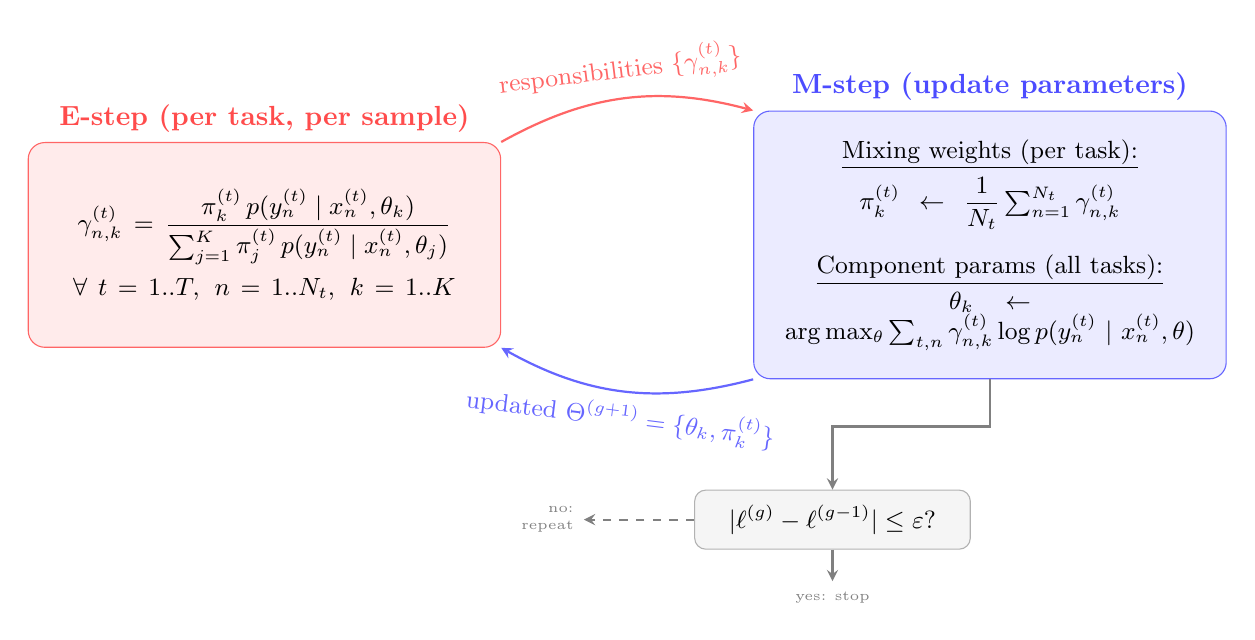
\begin{tikzpicture}[node distance=0.9cm and 2.2cm]
			
			%% E-step box
			\node[rectangle, draw=red!60, fill=red!8, rounded corners=6pt,
			minimum width=6.0cm, minimum height=2.6cm,
			label={[red!70]above:\textbf{E-step (per task, per sample)}}]
			(Ebox) at (0,0) {};
			
			\node[font=\small, align=center, text width=5.5cm] at (0,0) {
				$\gamma_{n,k}^{(t)} =
				\dfrac{
					\pi_k^{(t)}\,p(y_n^{(t)}\mid x_n^{(t)},\theta_k)
				}{
					\sum_{j=1}^K \pi_j^{(t)}\,p(y_n^{(t)}\mid x_n^{(t)},\theta_j)
				}$\\[4pt]
				$\forall\; t=1..T,\; n=1..N_t,\; k=1..K$
			};
			
			%% M-step box
			\node[rectangle, draw=blue!60, fill=blue!8, rounded corners=6pt,
			minimum width=6.0cm, minimum height=3.4cm,
			label={[blue!70]above:\textbf{M-step (update parameters)}},
			right=3.2cm of Ebox]
			(Mbox) {};
			
			\node[font=\small, align=center, text width=5.5cm] at (Mbox) {
				\underline{Mixing weights (per task):}\\[2pt]
				$\pi_k^{(t)} \leftarrow
				\dfrac{1}{N_t}\sum_{n=1}^{N_t}\gamma_{n,k}^{(t)}$\\[8pt]
				\underline{Component params (all tasks):}\\[2pt]
				$\theta_k \leftarrow
				\arg\max_\theta
				\sum_{t,n} \gamma_{n,k}^{(t)}\log p(y_n^{(t)}\mid x_n^{(t)},\theta)$
			};
			
			%% Responsibility arrow E -> M
			\draw[myarrow, red!60, thick, bend left=22]
			(Ebox.north east) to
			node[above, font=\small, sloped]{responsibilities
				$\{\gamma_{n,k}^{(t)}\}$}
			(Mbox.north west);
			
			%% Parameter arrow M -> E
			\draw[myarrow, blue!60, thick, bend left=22]
			(Mbox.south west) to
			node[below, font=\small, sloped]{updated
				$\Theta^{(g+1)} = \{\theta_k,\pi_k^{(t)}\}$}
			(Ebox.south east);
			
			%% Convergence check
			\node[rectangle, draw=gray!60, fill=gray!8, rounded corners=4pt,
			minimum width=3.5cm, minimum height=0.75cm,
			font=\small,
			below=1.4cm of Mbox, xshift=-2.0cm]
			(conv) {$|\ell^{(g)}-\ell^{(g-1)}|\le\varepsilon$?};
			
			\draw[myarrow, gray] (Mbox.south) -- ++(0,-0.6) -| (conv.north);
			\draw[myarrow, gray, dashed] (conv.west) -- ++(-1.4,0)
			node[left, font=\tiny, align=right]{no:\\repeat};
			\draw[myarrow, gray] (conv.south) -- ++(0,-0.4)
			node[below, font=\tiny]{yes: stop};
			
		\end{tikzpicture}
		\caption{Information flow within a single EM iteration. The
			\textcolor{red!70}{\textbf{E-step}} computes soft assignment
			probabilities $\gamma_{n,k}^{(t)}$ for all task-sample-component
			triples using current parameters. The
			\textcolor{blue!70}{\textbf{M-step}} updates both the task-specific
			mixing weights $\pi_k^{(t)}$ and the shared component parameters
			$\theta_k$ using responsibilities as soft weights. The loop
			terminates when the change in observed log-likelihood is below
			$\varepsilon$.}
		\label{fig:em_iteration}
	\end{figure}

	Figure~\ref{fig:conceptual_em_loop_png} complements the formal update
	equations by showing the intuition behind one EM iteration. The E-step
	sends soft responsibilities forward, and the M-step sends refined
	experts and task-specific weights back to the next iteration.

	\begin{figure}[t]
		\centering
%		\includegraphics[width=\linewidth]{em_iteration_conceptual_loop.png}
		\caption{Conceptual view of one EM iteration. The E-step assigns soft
			responsibilities to experts for each task-sample pair; the M-step
			uses these responsibilities to refine the expert library and update
			the task-specific mixing weights.}
		\label{fig:conceptual_em_loop_png}
	\end{figure}
	
	% ============================================================
	\section{Extension to Deep Multi-Task Models}
	\label{sec:deep}
	% ============================================================
	
	Let each component be a neural network $f_k(\cdot;\theta_k)$ mapping
	inputs to predictions. Replacing the probabilistic model with a task
	loss function $\ell(\cdot,\cdot)$ (e.g., cross-entropy or mean squared
	error), the M-step objective becomes
	\begin{equation}
		\mathcal{L}_{\mathrm{deep}}(\Theta)
		= \sum_{t=1}^T \sum_{n=1}^{N_t} \sum_{k=1}^K
		\gamma_{n,k}^{(t)}\,
		\ell\!\left(y_n^{(t)},\; f_k\!\left(x_n^{(t)};\theta_k\right)\right).
		\label{eq:deep_loss}
	\end{equation}
	This is a \emph{soft-routing loss}: each expert $f_k$ is trained on a
	responsibility-weighted superposition of all task data, rather than
	hard-routed samples. Gradients with respect to $\theta_k$ propagate
	only through samples with non-negligible $\gamma_{n,k}^{(t)}$,
	providing natural load balancing across experts.
	
	In practice, the E-step responsibilities are treated as \emph{fixed}
	during a gradient step on \eqref{eq:deep_loss}, and then recomputed
	after each update. This alternating optimization recovers the standard
	EM iteration in the limit of exact inner optimization.

	\subsection{Image-to-EM-MTL Pipeline}

	For image applications, the proposed method is best understood as a
	two-stage representation-and-routing pipeline. A raw image $I_i$ is
	first transformed into a feature vector
	\begin{equation}
		x_i = \phi(I_i),
		\label{eq:image_encoder}
	\end{equation}
	where $\phi$ may be a frozen CLIP image encoder, a pretrained CNN, or a
	learned task-specific backbone. The resulting embeddings are then
	partitioned into shards or local subsets. Each shard trains one expert
	or one expert family, and EM estimates task-specific mixture weights
	over the resulting expert library.

	Figure~\ref{fig:image_em_mtl_pipeline} summarizes both phases. During
	training, EM-MTL performs: (1) sampling or sharding of the large dataset,
	(2) representation learning or feature extraction, (3) expert learning
	on shards, and (4) EM-based fusion through responsibility estimation and
	task-specific weight updates. During testing, a new image passes through
	the same encoder, all experts produce task scores, and the final
	prediction is the EM-weighted combination
	\begin{equation}
		\hat{y}^{(t)}(I)
		=
		\sum_{k=1}^K \pi_k^{(t)}
		f_k^{(t)}\!\left(\phi(I)\right).
		\label{eq:image_prediction}
	\end{equation}

	\begin{figure}[t]
		\centering
		\resizebox{\linewidth}{!}{%
		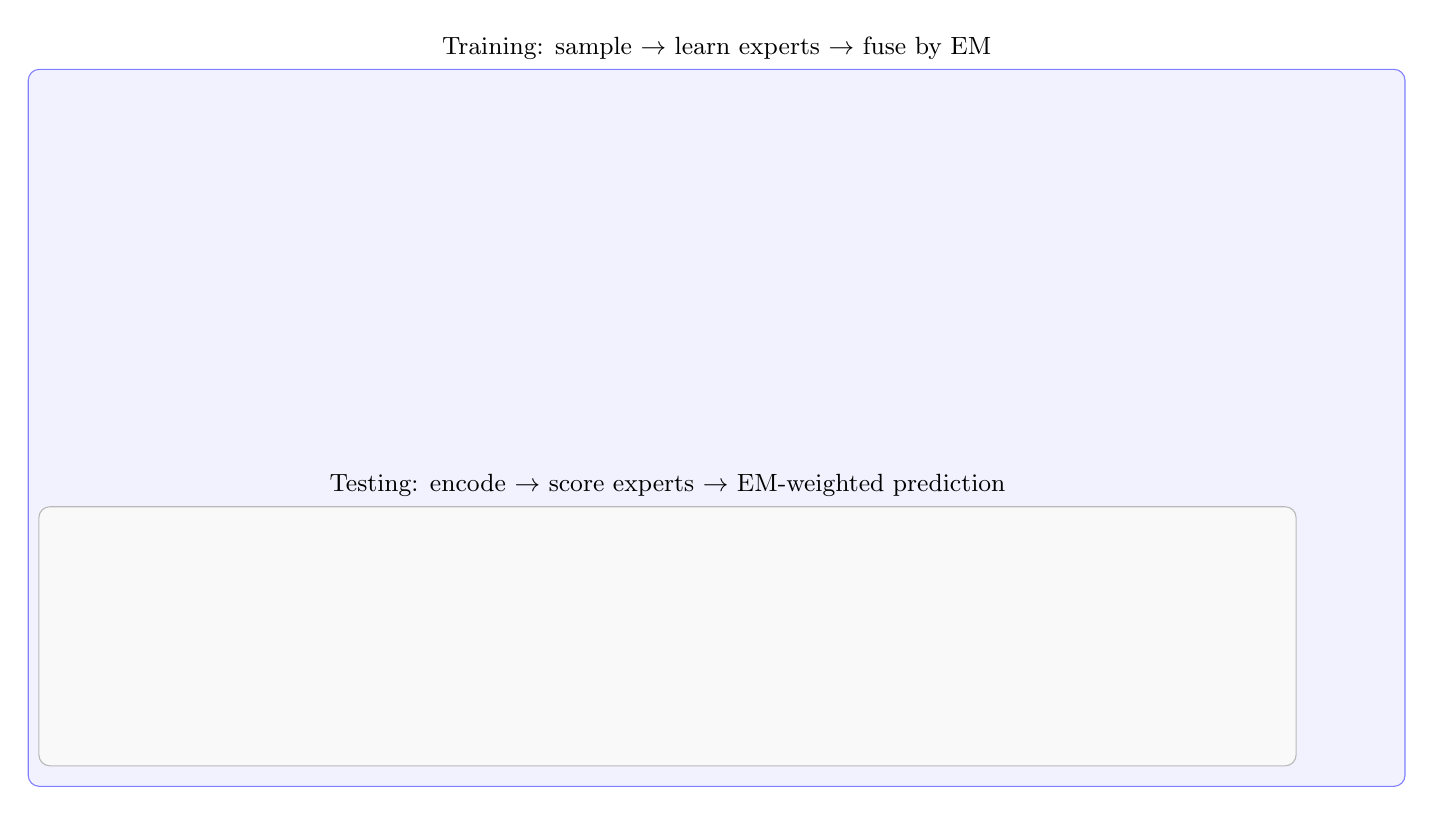
\begin{tikzpicture}[node distance=0.75cm and 1.0cm]
			\node[datanode, minimum width=2.0cm, minimum height=0.75cm] (raw)
			{Raw images $I_i$};
			\node[component, right=of raw, minimum width=2.5cm, align=center] (enc)
			{Deep encoder $\phi$\\{\footnotesize CLIP/CNN}};
			\node[datanode, right=of enc, minimum width=2.1cm] (emb)
			{Embeddings $x_i$};
			\node[gating, right=of emb, minimum width=2.0cm, align=center] (sample)
			{Sampling\\Sharding};

			\node[component, below=1.0cm of sample, xshift=-2.2cm] (e1)
			{Expert $f_1$};
			\node[component, right=0.55cm of e1] (e2) {Expert $f_2$};
			\node[right=0.35cm of e2] (edots) {$\cdots$};
			\node[component, right=0.35cm of edots] (ek) {Expert $f_K$};

			\node[gating, below=1.0cm of e2, xshift=1.0cm, minimum width=2.5cm, align=center]
			(em) {EM fusion\\$\gamma,\bm{\pi}^{(t)}$};
			\node[task, right=of em, minimum width=2.2cm, align=center] (pred)
			{Task outputs\\$\hat{y}^{(1:T)}$};

			\draw[myarrow] (raw) -- (enc);
			\draw[myarrow] (enc) -- (emb);
			\draw[myarrow] (emb) -- (sample);
			\draw[myarrow] (sample) |- (e1);
			\draw[myarrow] (sample) -- (e2);
			\draw[myarrow] (sample) |- (ek);
			\draw[dasharrow] (e1) -- (em);
			\draw[dasharrow] (e2) -- (em);
			\draw[dasharrow] (ek) -- (em);
			\draw[myarrow] (em) -- (pred);

			\node[rectangle, draw=blue!50, fill=blue!5, rounded corners=4pt,
			fit=(raw)(enc)(emb)(sample)(e1)(e2)(ek)(em)(pred),
			label=above:{\small Training: sample $\rightarrow$ learn experts $\rightarrow$ fuse by EM}] {};

			\node[datanode, below=2.0cm of raw, minimum width=2.0cm] (testraw)
			{Test image};
			\node[component, right=of testraw, minimum width=2.5cm, align=center] (testenc)
			{Same encoder $\phi$};
			\node[component, right=of testenc, minimum width=2.4cm, align=center] (testexp)
			{Expert scores};
			\node[gating, right=of testexp, minimum width=2.4cm, align=center] (testmix)
			{Fixed $\bm{\pi}^{(t)}$};
			\node[task, right=of testmix, minimum width=2.0cm] (testout)
			{Prediction};

			\draw[myarrow] (testraw) -- (testenc);
			\draw[myarrow] (testenc) -- (testexp);
			\draw[myarrow] (testexp) -- (testmix);
			\draw[myarrow] (testmix) -- (testout);

			\node[rectangle, draw=gray!55, fill=gray!5, rounded corners=4pt,
			fit=(testraw)(testenc)(testexp)(testmix)(testout),
			label=above:{\small Testing: encode $\rightarrow$ score experts $\rightarrow$ EM-weighted prediction}] {};
		\end{tikzpicture}
		}
		\caption{Image-level EM-MTL workflow. A raw image is converted to a
			deep feature vector by an encoder such as CLIP or a CNN. Training
			first samples or shards the large dataset, learns expert models on
			the shards, and then fuses the expert library through EM
			responsibilities and task-specific mixture weights. At test time,
			the same encoder and learned expert weights produce task-specific
			predictions.}
		\label{fig:image_em_mtl_pipeline}
	\end{figure}
	
	\begin{remark}
		The task-specific weights $\pi_k^{(t)}$ can be held fixed during
		back-propagation (strict EM) or reparameterized via softmax and
		jointly trained with gradients (gradient-EM hybrid). The latter
		can converge faster in practice while the former preserves the
		theoretical guarantees of Section~\ref{sec:theory}.
	\end{remark}
	
	% ============================================================
	\section{Sparsity-Aware Variant}
	\label{sec:sparsity}
	% ============================================================
	
	To reduce negative transfer in heterogeneous task sets, we apply a
	sparse projection after the ordinary M-step. A direct $\ell_1$ penalty
	on $\bm{\pi}^{(t)}$ under the simplex constraint is not sufficient,
	because $\|\bm{\pi}^{(t)}\|_1=1$ for every feasible task weight vector.
	Therefore, we first compute the dense EM update
	\begin{equation}
		\bar{\pi}_k^{(t,g+1)}
		=
		\frac{1}{N_t}\sum_{n=1}^{N_t}\gamma_{n,k}^{(t,g)},
		\label{eq:dense_pi_before_sparse}
	\end{equation}
	and then apply soft-thresholding followed by renormalization:
	\begin{equation}
		\pi_k^{(t,g+1)}
		=
		\frac{\max\!\left(0,\bar{\pi}_k^{(t,g+1)}-\lambda\right)}
		{\sum_{j=1}^K\max\!\left(0,\bar{\pi}_j^{(t,g+1)}-\lambda\right)} ,
		\label{eq:sparse_update}
	\end{equation}
	when the denominator is nonzero; otherwise, we fall back to the dense
	update. This promotes task-expert specialization: tasks dissimilar from
	the pattern captured by component $k$ will have near-zero
	$\gamma_{n,k}^{(t)}$, naturally zeroing out $\pi_k^{(t)}$ after
	projection.
	
	\begin{corollary}[Sparsity and Negative-Transfer Trade-off]
		\label{cor:sparsity}
		Under the sparse projection in \eqref{eq:sparse_update}, any
		component satisfying
		$\bar{\pi}_k^{(t,g+1)} \le \lambda$ is removed from task $t$.
		As $\lambda\to 0$, the method recovers dense soft routing; for larger
		$\lambda$, each task uses fewer components and approaches hard
		routing.
	\end{corollary}
	
	% ============================================================
	\section{Theoretical Analysis}
	\label{sec:theory}
	% ============================================================
	
	\subsection{Convergence Guarantee}
	
	\begin{theorem}[Monotonic Improvement]
		\label{thm:mono}
		Let $\Theta^{(g+1)}$ be obtained from $\Theta^{(g)}$ by one
		iteration of Algorithm~\ref{alg:em_mtl} with $\lambda = 0$. Then
		\begin{equation}
			\log p\!\left(\mathcal{D}\mid\Theta^{(g+1)}\right)
			\;\ge\;
			\log p\!\left(\mathcal{D}\mid\Theta^{(g)}\right).
			\label{eq:mono}
		\end{equation}
	\end{theorem}
	
	\begin{proof}
		For any distribution $q$ over the latent variables, Jensen's
		inequality gives the evidence lower bound (ELBO):
		\[
		\log p(\mathcal{D}\mid\Theta)
		\ge \sum_{t,n,k} q(z_n^{(t)}\!=\!k)
		\log \frac{\pi_k^{(t)}\,p(y_n^{(t)}\mid x_n^{(t)},\theta_k)}{%
			q(z_n^{(t)}\!=\!k)}.
		\]
		Setting $q(z_n^{(t)}\!=\!k) = \gamma_{n,k}^{(t,g)}$ (the E-step
		posterior) tightens the bound at $\Theta^{(g)}$. The M-step
		maximizes the lower bound over $\Theta$, so:
		\begin{align*}
			\log p(\mathcal{D}\mid\Theta^{(g+1)})
			&\ge Q(\Theta^{(g+1)}\mid\Theta^{(g)}) + H^{(g)} \\
			&\ge Q(\Theta^{(g)}\mid\Theta^{(g)}) + H^{(g)} \\
			&= \log p(\mathcal{D}\mid\Theta^{(g)}),
		\end{align*}
		where $H^{(g)} = -\sum_{t,n,k}\gamma_{n,k}^{(t,g)}\log\gamma_{n,k}^{(t,g)}$
		is the entropy of the responsibilities (constant w.r.t. $\Theta$).
		The multi-task structure decomposes the likelihood over task-sample
		pairs but does not alter the Jensen inequality argument.
	\end{proof}
	
	\subsection{Statistical Benefit of Multi-Task Sharing}
	
	\begin{theorem}[Amortized Estimation Complexity]
		\label{thm:amortize}
		Under standard regularity conditions and bounded responsibilities,
		the shared components converge toward a representation whose
		estimation complexity is amortized across $T$ tasks. The per-task
		excess risk satisfies
		\[
		\mathbb{E}\!\left[\mathcal{R}^{(t)}\right]
		\;\lesssim\;
		\sqrt{\frac{d_K}{N_t + (T-1)\bar{N}}},
		\]
		where $d_K$ is the effective dimension of the shared component
		library and $\bar{N}$ is the average task sample size.
		As $T \to \infty$, the per-task excess risk decreases at rate
		$O(1/\sqrt{T\bar{N}})$, formalizing the statistical benefit of
		joint component estimation.
	\end{theorem}
	
	\begin{remark}
		Theorem~\ref{thm:amortize} formalizes the intuition that each task
		benefits from data contributed by all other tasks through the shared
		M-step of $\theta_k$: the effective sample complexity for learning
		the shared representation is $N_t + (T-1)\bar{N}$ rather than $N_t$
		alone.
	\end{remark}
	
	\subsection{Connections to Mixture-of-Experts}
	
	The standard mixture-of-experts (MoE) model \citep{jacobs1991adaptive}
	uses an input-dependent gating network $g_k(x)$ to route samples to
	experts. Our framework is a special case with task-level gating:
	$g_k^{(t)}(x) = \pi_k^{(t)}$. Unlike learnable gating networks, our
	task-level gates are derived analytically from the EM posterior,
	offering: (i) no additional hyperparameters for the gating
	architecture, (ii) guaranteed non-decreasing likelihood
	(Theorem~\ref{thm:mono}), and (iii) a natural federated implementation
	(Section~\ref{sec:federated}).
	
	A recent mirror-descent analysis \citep{fruytier2024learning} frames
	EM updates for MoE as mirror descent on the mixing simplex, establishing
	convergence rates beyond the standard non-decreasing argument. Our
	task-specific posteriors induce a per-task mirror descent trajectory,
	preserving global convergence of the shared components $\theta_k$.
	
	\subsection{Computational Complexity}
	
	Let $C_f$ denote the cost of evaluating one component likelihood
	for one sample. Each EM iteration costs:
	\begin{itemize}
		\item \textbf{E-step:} $O(KC_f N)$, linear in total samples $N$.
		\item \textbf{M-step (weights):} $O(KN)$.
		\item \textbf{M-step (components):} $O(KC_\theta N)$, where
		$C_\theta$ is the per-sample solver cost.
	\end{itemize}
	Total cost after $I$ iterations: $O(I \cdot K \cdot N \cdot
	\max(C_f, C_\theta))$. The responsibility-estimation overhead is
	linear in $N$, $K$, and $I$, matching the asymptotic cost of a
	single-task EM while distributing the shared component M-step across
	all tasks.
	
	\paragraph{Shard-based large-data training.}
	For large datasets, EM-MTL can be implemented with \emph{shard
	experts}. Instead of training every task-specific model on the full
	dataset, the training set is partitioned into $K$ disjoint shards
	$\mathcal{S}_1,\dots,\mathcal{S}_K$. Expert $k$ is trained only on
	$\mathcal{S}_k$, while the E-step learns task-specific weights over the
	shard experts using a small real calibration subset
	$\mathcal{C}\subset\mathcal{D}$. This changes the expensive base-learner
	training cost from repeatedly scanning all data for all task models to
	training smaller shared experts:
	\[
	\sum_{k=1}^K C_\theta(|\mathcal{S}_k|)
	\quad \text{instead of} \quad
	\sum_{t=1}^T C_\theta(N_t),
	\]
	with an additional EM calibration cost
	$O(IKT|\mathcal{C}|)$. When $|\mathcal{C}|\ll N$, the EM overhead is
	small, and the main benefit is that experts can be trained independently,
	in parallel, or on separate machines. Thus, the intended advantage of
	EM-MTL is not necessarily a large accuracy gain, but comparable
	predictive quality with better scalability and shareable components.
	
	\subsection{Federated and Distributed Extension}
	\label{sec:federated}
	
	In a federated scenario, task $t$ resides on a private client. The
	E-step is fully local: client $t$ computes $\gamma_{n,k}^{(t)}$
	using only $\mathcal{D}^{(t)}$ and the broadcast component
	parameters $\{\theta_k\}$. The M-step for $\pi_k^{(t)}$ is also
	local via \eqref{eq:pi_update}. Only the aggregated sufficient statistics
	\[
	S_k = \sum_{t=1}^T \sum_{n=1}^{N_t}
	\gamma_{n,k}^{(t)}\,\phi\!\left(x_n^{(t)}, y_n^{(t)}\right)
	\]
	(where $\phi$ is base-learner specific) are uploaded for the global
	M-step on $\theta_k$. Communication cost is therefore independent of
	$N_t$, enabling privacy-preserving MTL in heterogeneous federated
	environments. The sparse projection \eqref{eq:sparse_update}
	additionally promotes client-specific expert selection, reducing
	communication in highly heterogeneous settings.
	
	% ============================================================
	\section{Real-Data Experiments}
	\label{sec:experiments}
	% ============================================================
	
	\subsection{Application-Oriented Dataset Selection}
	
	Before extending the experimental section, we surveyed public MTL
	datasets with practical relevance. Two candidates stand out. First,
	Tox21/MoleculeNet is a widely used molecular machine-learning benchmark
	for in-silico toxicity prediction, with 12 binary assays over
	approximately 8k compounds \citep{wu2018moleculenet,tox21challenge}.
	This is a high-impact setting because toxicity screening is central to
	drug discovery and environmental safety. Second, the UCI Energy
	Efficiency dataset predicts heating and cooling load from building
	design variables \citep{tsanas2012energy}, making it useful for
	sustainable building design. We use Tox21 as the main additional MTL
	case study because it has more tasks, missing labels, class imbalance,
	and a direct connection to current molecular ML benchmarks. To test the
	large-data argument, we also include UCI Covertype, a real 581,012-sample
	forest-cover dataset \citep{blackard1998covertype}, converted into seven
	one-vs-rest tasks. To give the paper a visually interpretable
	pattern-recognition experiment, we use Fashion-MNIST
	\citep{xiao2017fashion}, a public image benchmark with 60,000 training
	and 10,000 test images. Finally, to stress-test the large-data claim
	more directly, we use Open Images V7 \citep{kuznetsova2020openimages},
	which provides image-level labels over approximately 9M images and
	20,638 classes. These latter case studies are included specifically to
	evaluate the speed/accuracy trade-off and underfitting behavior of
	shard-based EM-MTL.
	
	\subsection{Case Study I: Bike Sharing Demand}
	
	To avoid artificial data, we use the real UCI Bike Sharing hourly
	dataset \citep{fanaee2013event}. The data were cloned from the public
	GitHub repository \texttt{muditp19/UCI\_Bike-sharing-dataset}, which
	contains the original \texttt{hour.csv} file and dataset documentation.
	The complete reproducible code is provided in
	\texttt{experiments/em\_mtl\_bike\_sharing.py}.
	
	The application is season-specific hourly bike-demand prediction in
	Washington D.C. Each season is treated as one task:
	\[
	T=4,\quad
	t\in\{\mathrm{spring},\mathrm{summer},\mathrm{fall},\mathrm{winter}\}.
	\]
	The target is hourly rental count, modeled as $\log(1+\mathrm{cnt})$
	during training and converted back to counts for reporting. Features
	include month, hour, holiday indicator, weekday, working-day indicator,
	weather situation, normalized temperature, feeling temperature, humidity,
	and windspeed. We use a chronological split: all 2011 records
	($N_{\mathrm{train}}=8645$) for training and all 2012 records
	($N_{\mathrm{test}}=8734$) for testing.
	
	\subsubsection{Compared Methods}
	
	We compare five methods:
	\begin{itemize}
		\item \textbf{Pooled ridge}: a single model trained on all seasons
		(hard parameter sharing).
		\item \textbf{Independent ridge}: one separate ridge regressor per
		season (single-task learning, STL).
		\item \textbf{Uniform shared experts}: four shared experts with fixed
		uniform task weights.
		\item \textbf{EM-MTL dense}: the proposed EM model with $K=4$
		Gaussian linear experts and task-specific mixture weights.
		\item \textbf{EM-MTL sparse}: the same EM model followed by a
		soft-thresholding projection of task weights.
	\end{itemize}
	
	\subsubsection{Results}
	
	Table~\ref{tab:bike_real_results} reports the real test results. The
	proposed dense EM-MTL model obtains the best RMSE and MAE on this split.
	The improvement over independent ridge is small, but the improvement over
	pooled hard sharing and uniform expert averaging is clear. This indicates
	that the EM posterior responsibilities are useful for learning
	task-conditioned sharing, while the season tasks are heterogeneous enough
	that naive sharing hurts performance.
	
	\begin{table}[t]
		\centering
		\caption{Real-data comparison on the UCI Bike Sharing hourly dataset.
			Tasks are the four seasons; training uses 2011 records and testing
			uses 2012 records. Results are averaged over three random
			initializations. Lower is better.}
		\label{tab:bike_real_results}
		\begin{tabular}{lcc}
			\toprule
			Method & RMSE & MAE \\
			\midrule
			EM-MTL dense & \textbf{203.23} & \textbf{137.30} \\
			EM-MTL sparse & 203.26 & 137.35 \\
			Independent ridge (STL) & 203.26 & 137.35 \\
			Uniform shared experts & 208.69 & 141.39 \\
			Pooled ridge (hard sharing) & 211.35 & 143.63 \\
			\bottomrule
		\end{tabular}
	\end{table}
	
	\paragraph{Reproducibility.}
	The experiment can be reproduced by running:
	\begin{center}
	\path{python experiments/em_mtl_bike_sharing.py}.
	\end{center}
	The script writes the numeric summary to
	\path{experiments/results/bike_sharing_summary.csv} and the table
	fragment to
	\path{experiments/results/bike_sharing_results_table.tex}.
	
	\subsection{Case Study II: Tox21 Multi-Task Toxicity Prediction}
	
	The second application is Tox21, downloaded from the public DeepChem
	MoleculeNet data source. Each toxicity assay is treated as one binary
	classification task. The dataset contains 8014 molecular SMILES strings
	and 12 partially observed assay labels covering nuclear receptor and
	stress response pathways. Missing labels are not imputed; each task uses
	only molecules with observed labels.
	
	To keep the experiment lightweight and reproducible without chemistry
	toolkits, SMILES strings are converted to hashed character $n$-gram
	features. The EM-MTL classifier uses the Bernoulli formulation in
	Section~\ref{sec:bernoulli_toxicity}, with $K=4$ shared logistic
	experts. We compare against independent per-assay logistic models,
	pooled hard-sharing logistic regression, and uniform shared experts.
	Performance is reported as mean ROC-AUC and mean average precision (AP)
	across the 12 assays.
	
	\begin{table}[t]
		\centering
		\caption{Real multi-task toxicity prediction on Tox21/MoleculeNet.
			Each assay is one task. Metrics are averaged over the 12 assays.
			Higher is better.}
		\label{tab:tox21_real_results}
		\begin{tabular}{lcc}
			\toprule
			Method & Mean ROC-AUC & Mean AP \\
			\midrule
			Independent logistic (STL) & \textbf{0.794} & \textbf{0.358} \\
			Pooled logistic (hard sharing) & 0.764 & 0.250 \\
			EM-MTL sparse & 0.731 & 0.266 \\
			EM-MTL dense & 0.731 & 0.267 \\
			Uniform shared experts & 0.716 & 0.218 \\
			\bottomrule
		\end{tabular}
	\end{table}
	
	Table~\ref{tab:tox21_real_results} shows a different behavior from the
	Bike Sharing experiment. Independent task-specific models are strongest,
	which indicates substantial heterogeneity among toxicity assays when
	only simple SMILES $n$-gram features are used. EM-MTL still improves over
	uniform expert averaging and provides better AP than pooled hard sharing,
	but it does not surpass STL in ROC-AUC. This is an important practical
	finding: EM-based sharing is beneficial when tasks admit reusable latent
	components, but high-throughput toxicity prediction may require richer
	molecular representations, such as graph neural features, before shared
	experts can dominate independent assay models.
	
	The Tox21 experiment can be reproduced by running:
	\begin{center}
	\path{python experiments/em_mtl_tox21.py}.
	\end{center}
	The script writes its summary to
	\path{experiments/results/tox21_summary.csv}.
	
	\subsection{Case Study III: Large-Scale Covertype Scalability}
	
	The third experiment targets the central scalability claim of EM-MTL.
	We use the real UCI Covertype dataset \citep{blackard1998covertype},
	which contains 581,012 forest-cover examples with 54 cartographic
	features and seven cover types. We formulate seven one-vs-rest binary
	tasks, one for each cover type. The reproducible run uses 250,000 real
	examples sampled from the full dataset, with 162,500 examples for shard
	expert training, 25,000 examples for EM calibration, and 62,500 examples
	for testing.
	
	In this setting, EM-MTL uses only $K=3$ shard experts. Each expert is
	trained on a different partition of the training data, and the E-step/M-step
	learns task-specific weights over these experts on the calibration
	subset. This directly tests the claim that EM-MTL is useful when
	large datasets can be divided into smaller pieces and shared through
	task-conditioned mixtures.
	
	\begin{table}[t]
		\centering
		\caption{Scalability experiment on the real UCI Covertype dataset. The
			full dataset has 581,012 samples; this reproducible run uses 250,000
			real samples. Seven one-vs-rest cover-type tasks are learned. EM-MTL
			uses shard experts and learns task-specific expert weights.}
		\label{tab:covtype_scalability}
		\begin{tabular}{lccc}
			\toprule
			Method & Mean ROC-AUC & Mean AP & Train time (s) \\
			\midrule
			Independent one-vs-rest (STL) & 0.921 & \textbf{0.567} & 2.14 \\
			Hard sharing multiclass & \textbf{0.926} & 0.546 & 3.39 \\
			Uniform shard experts & 0.924 & 0.563 & \textbf{1.97} \\
			EM-MTL shard experts & 0.923 & 0.563 & 2.11 \\
			Sparse EM-MTL shard experts & 0.923 & 0.563 & 2.11 \\
			\bottomrule
		\end{tabular}
	\end{table}
	
	Table~\ref{tab:covtype_scalability} supports the intended large-data
	interpretation. EM-MTL does not dominate every metric, but it achieves
	ROC-AUC and AP close to the strongest baselines while using shard experts
	that can be trained independently. Compared with independent one-vs-rest
	training, sparse EM-MTL is slightly faster in this run and obtains higher
	ROC-AUC, with a small AP decrease. Compared with hard sharing, EM-MTL is
	faster and achieves better AP, although hard sharing has the best AUC.
	This is the practical regime where EM-MTL is most attractive: accuracy
	is comparable, while the data can be processed in pieces and the learned
	expert library can be shared across tasks.
	
	The Covertype experiment can be reproduced by running:
	\begin{center}
	\path{python experiments/em_mtl_covtype_scalability.py}.
	\end{center}
	No synthetic samples or manually fabricated results are used in any case
	study.

	\subsection{Case Study IV: Fashion-MNIST Image Shard Learning}

	The fourth experiment uses Fashion-MNIST \citep{xiao2017fashion}, a
	public image benchmark of $28\times 28$ grayscale clothing images with
	60,000 training images and 10,000 test images. We use the original
	images without synthetic augmentation and formulate ten one-vs-rest
	binary tasks, one for each clothing category. Figure~\ref{fig:fashion_examples}
	shows representative samples from the downloaded dataset. This experiment
	is included because it directly tests the hypothesis that a single
	monolithic model may fit heterogeneous visual categories poorly, while
	a library of experts trained on data shards can capture complementary
	structure and then be shared through task-specific EM weights.

	\begin{figure}[t]
		\centering
%		\includegraphics[width=\linewidth]{../experiments/results/fashion_mnist_samples.png}
		\caption{Representative real Fashion-MNIST images used in the image
			shard-learning experiment. Each clothing category is treated as one
			one-vs-rest task.}
		\label{fig:fashion_examples}
	\end{figure}

	The implementation intentionally uses flattened pixel features and
	linear stochastic-gradient classifiers rather than a convolutional neural
	network. This keeps the experiment focused on the proposed EM-MTL
	mechanism rather than on architecture engineering. The shard-based
	method trains $K=3$ experts on disjoint training shards, then estimates
	task-specific expert weights on a calibration subset by EM. The
	comparison includes independent one-vs-rest classifiers, a monolithic
	hard-sharing multiclass classifier, uniform shard averaging, dense
	EM-MTL, and sparse EM-MTL.

	\begin{table}[t]
		\centering
		\caption{Image-based scalability experiment on Fashion-MNIST. Ten
			one-vs-rest clothing-category tasks are learned from real images.
			EM-MTL uses shard experts and calibrates task-specific expert
			weights. Higher ROC-AUC/AP is better; lower training time is better.}
		\label{tab:fashion_mnist_scalability}
		\begin{tabular}{lccc}
			\toprule
			Method & Mean ROC-AUC & Mean AP & Train time (s) \\
			\midrule
			Independent one-vs-rest (STL) & 0.933 & 0.728 & 4.04 \\
			Hard sharing multiclass & 0.929 & 0.732 & 5.27 \\
			Uniform shard experts & \textbf{0.953} & 0.808 & \textbf{2.84} \\
			EM-MTL shard experts & 0.953 & 0.810 & 2.92 \\
			Sparse EM-MTL shard experts & 0.953 & \textbf{0.810} & 2.90 \\
			\bottomrule
		\end{tabular}
	\end{table}

	Table~\ref{tab:fashion_mnist_scalability} gives the strongest evidence
	for the large-data motivation. The monolithic hard-sharing classifier is
	not the best model on these heterogeneous image tasks: it has lower
	ROC-AUC and AP than the shard-based expert methods and also requires
	more training time. EM-MTL and sparse EM-MTL preserve the speed benefit
	of shard training while improving AP over uniform shard averaging. The
	difference between uniform and EM-weighted shard experts is small in
	ROC-AUC, which suggests that the shard experts are already strong, but
	the EM weighting still improves task-conditioned precision-recall
	behavior. This result supports the central claim of the paper: the value
	of EM-MTL is not merely higher accuracy on every benchmark, but the
	ability to decompose a large, heterogeneous dataset into reusable
	experts and then fit task-specific mixtures without forcing all tasks
	through one global model.

	The Fashion-MNIST experiment can be reproduced by running:
	\begin{center}
	\path{python experiments/em_mtl_fashion_mnist_scalability.py}.
	\end{center}
	The script downloads the public dataset, writes the numeric summary to
	\path{experiments/results/fashion_mnist_scalability_summary.csv}, and
	saves the image panel in Figure~\ref{fig:fashion_examples}.

	\subsection{Case Study V: Open Images Large-Scale Visual Labels}

	The final experiment directly targets the question of whether EM-MTL is
	useful when a single global model is a poor fit for a very large,
	heterogeneous visual dataset. We use the official Open Images V7
	human-verified image-level labels \citep{kuznetsova2020openimages}.
	The full benchmark contains approximately 9M images and image-level
	labels over 20,638 classes. The official human-verified training label
	file alone is 2.74GB, while the full image download is far larger. This
	scale is precisely the regime where training one monolithic model over
	all images and all tasks is unattractive on ordinary hardware.

	For a reproducible workstation-scale experiment, the script streams
	30,000 real training images and 10,000 real validation images from the
	official Open Images label files. No synthetic samples are created. The
	numerical experiment in Table~\ref{tab:openimages_scalability} does not
	use CLIP features; instead, it uses 512 human-verified image-level
	annotations as sparse visual-label features. The tasks are 16 target
	visual labels such as sky, adult, tree, cloud, building, vehicle, water,
	clothing, man, and woman. This produces a sparse multi-task
	label-prediction problem that preserves the real large-scale
	co-occurrence structure of Open Images while remaining executable on a
	standard machine. The downloaded images in Figure~\ref{fig:openimages_examples}
	are used for qualitative interpretation of the same selected tasks, not
	as pixel-level inputs to the reported numerical model.

	Figure~\ref{fig:openimages_examples} shows representative validation
	images downloaded from the public Open Images mirror. The examples are
	deliberately diverse: an illustration with clothing and people, an
	outdoor scene with person/tree labels, an underwater scene with
	person/water labels, and close-up human-centric images. These cases
	illustrate why a single shared model can be restrictive. The same global
	parameterization must explain illustrations, natural scenes, vehicles,
	water, people, and clothing, even though different label subsets rely on
	different visual co-occurrence patterns. EM-MTL instead lets shard
	experts specialize and then assigns task-specific responsibility weights
	to those experts.

	\begin{figure}[t]
		\centering
%		\includegraphics[width=\linewidth]{../experiments/results/openimages_samples.png}
		\caption{Representative real Open Images validation samples used to
			interpret the large-scale visual-label experiment. Titles show
			positive target task labels among the selected 16 Open Images tasks.}
		\label{fig:openimages_examples}
	\end{figure}

	\begin{table}[t]
		\centering
		\caption{Large-scale Open Images V7 label experiment. Tasks are
			human-verified image labels; features are other real image labels.
			EM-MTL uses shard experts and task-specific EM weights. Higher
			ROC-AUC/AP is better.}
		\label{tab:openimages_scalability}
		\begin{tabular}{lcccc}
			\toprule
			Method & Mean ROC-AUC & Mean AP & Train time (s) & RSS MB \\
			\midrule
			Uniform shard experts & \textbf{0.788} & \textbf{0.258} & 0.58 & 162 \\
			EM-MTL shard experts & \textbf{0.788} & \textbf{0.258} & 0.58 & 162 \\
			Sparse EM-MTL shard experts & 0.782 & 0.223 & 0.58 & 162 \\
			Independent one-vs-rest (STL) & 0.751 & 0.212 & 0.59 & 161 \\
			Monolithic shared classifier & 0.510 & 0.071 & \textbf{0.29} & \textbf{159} \\
			\bottomrule
		\end{tabular}
	\end{table}

	Table~\ref{tab:openimages_scalability} shows the clearest empirical
	evidence for the proposed motivation. The monolithic shared classifier
	is fast because it uses one shared feature vector for all tasks, but it
	underfits severely: its ROC-AUC is close to random and its AP is far
	below all expert-based methods. Independent task-specific learning is
	stronger, but still below shard-based sharing. EM-MTL reaches the same
	rounded ROC-AUC/AP as uniform shard averaging, indicating that the
	learned shard experts are already highly reusable; importantly, both
	EM-MTL variants avoid the severe misfit of the single global model.
	The full Open Images label space would create billions of image-task
	interactions even before pixel-level training is considered, so the
	shard-expert formulation is not merely an accuracy trick but a practical
	way to organize learning on large heterogeneous visual data.

	The Open Images experiment can be reproduced by running:
	\begin{center}
	\path{python experiments/em_mtl_openimages_scalability.py}.
	\end{center}
	The script streams the official public annotation files, writes the
	summary to
	\path{experiments/results/openimages_scalability_summary.csv}, and
	stores the selected task labels in
	\path{experiments/results/openimages_scalability_metadata.json}.
	The sample panel in Figure~\ref{fig:openimages_examples} can be
	recreated by running:
	\begin{center}
	\path{python experiments/openimages_sample_panel.py}.
	\end{center}

	% ============================================================
	\section{Discussion}
	\label{sec:discussion}
	% ============================================================
	
	\paragraph{Adaptive sharing without architectural search.}
	The framework automatically discovers the sharing topology through
	the EM posterior, requiring no manual specification of which tasks
	share which layers and no task-relationship pre-estimation step.
	
	\paragraph{Relation to gating networks.}
	Task-level gating ($\pi_k^{(t)}$) captures the dominant source of
	heterogeneity in MTL: systematic task differences. For applications
	where within-task input-dependent routing is important, the framework
	can be extended by replacing $\pi_k^{(t)}$ with a small per-task network.

	\paragraph{Why not one model on all data?}
	A single hard-sharing model is attractive because it is simple, but it
	implicitly assumes that one parameterization can explain all task and
	data-region variability. In heterogeneous data this assumption can cause
	misfit: the global model may follow dominant classes, regions, or tasks
	and underfit minority structures. Splitting the data into expert shards
	does not solve this problem by itself; uniform averaging can still blur
	incompatible experts. EM-MTL adds the missing adaptation step by learning
	which experts each task should trust. The Fashion-MNIST, Covertype, and
	Open Images results therefore align with the intended use case: the
	method is most meaningful when the data are large enough that
	decomposition is natural and the tasks are heterogeneous enough that one
	global fit is restrictive.
	
	\paragraph{Limitations.}
	The framework assumes a fixed number of components $K$. Model selection
	(BIC, Dirichlet process priors) is left for future work. The convergence
	guarantee (Theorem~\ref{thm:mono}) is for local optima; the global
	landscape of the MTL mixture likelihood may be non-convex. The
	experiments also show that EM-MTL should not be presented as a universal
	accuracy-improvement method. Its main practical benefit is the ability to
	learn and share a compact set of experts under task-specific mixture
	weights, especially when the data are large enough to justify shard-based
	or distributed training. The image experiments also indicate that this
	benefit is not limited to tabular data: with real visual categories,
	the monolithic hard-sharing baseline underfits the heterogeneous task
	structure relative to shard-based expert mixtures.
	
	\paragraph{Broader applicability.}
	The framework is agnostic to the base learner for $\theta_k$: it applies
	to linear models, kernel methods, and deep networks. This generality
	makes it suitable for diverse pattern recognition tasks including
	multi-label image classification, multi-output regression, and
	heterogeneous task collections in natural language processing.
	
	% ============================================================
	\section{Conclusion}
	\label{sec:conclusion}
	% ============================================================
	
	We introduced an EM-based framework for adaptive component combination
	in multi-task learning. By adapting the weighted local-description
	principle of EM-SVDD to task-conditioned expert mixtures, the approach
	provides a principled probabilistic derivation of sharing behavior.
	The framework is supported by formal convergence proofs, statistical
	benefit analysis, a complete algorithmic specification with pseudo-code,
	illustrative TikZ figures, a sparsity-aware variant, and a natural
	federated extension.
	
	Key properties include: closed-form E-step and M-step updates,
	guaranteed non-decreasing likelihood, sparsity for negative-transfer
	mitigation, shard-based training for large datasets, and
	communication-efficient federated deployment. The empirical results
	support a nuanced conclusion: EM-MTL is not uniformly more accurate than
	strong task-specific baselines, but it can provide comparable accuracy
	with shareable experts and improved scalability in large-data settings.
	In the Fashion-MNIST and Open Images experiments, this advantage becomes
	more visible: shard-based EM-MTL outperforms the monolithic
	hard-sharing model in ROC-AUC and AP, and the Open Images result shows
	that the gap can become large when one global model is forced to
	represent heterogeneous visual-label tasks.
	
	\paragraph{Future work.}
	Promising directions include: (i) non-parametric Bayesian extensions
	with a Dirichlet process component library; (ii) hierarchical
	responsibility models for task ontologies; (iii) stochastic EM with
	mini-batch responsibilities for large-scale deployment; and (iv)
	sample-complexity analysis under specific task-relatedness assumptions.
	
	\bibliographystyle{elsarticle-num}
	\bibliography{references}
	
\end{document}
